% ========================
% # Manual de Febradas   #
% ========================

\subsubsection{Manual de Febradas}

Fazer uma febrada parece a coisa mais simples do mundo e a verdade é que não é algo muito difícil. No entanto, falham sempre vários pequenos pormenores no decorrer das febras que são cruciais para o seu sucesso como, entre vários casos, por exemplo a falta de carvão no início das febradas, hora que costuma culminar com a saída das pessoas das aulas e, como tal, com a hora de maior afluência onde é fulcral ter o maior número de febras prontas para vender e garantir que a febrada tem retorno.

Assim, serve o presente guião para colmatar todas as possíveis falhas que possam ocorrer na preparação de uma febrada.

\paragraph{O que é necessário?}
Antes de mais, é preciso que exista um espaço para realizar o evento, daí ser necessário fazer o pedido de autorização de espaço. Para isso basta enviar um e-mail ao Diretor do Departamento com todas as informações do evento (data, hora e motivo), fazendo sempre referência ao comprometimento em deixar o espaço limpo e arrumado.

Posto isto é necessário fazer a “To-Do List”:
\begin{itemize}
    \item Compras
    \begin{itemize}
        \item Pão: a encomenda é feita normalmente na Padaria do Alto de S. João (239 714 313), ao lado do Pingo Doce da Portela. O preço é de 8 cêntimos/pão sendo, no entanto, necessário mencionar que a encomenda é para o \acrshort{neeec} e não é passada fatura. É também possível fazer a encomenda junto da Padaria onde o Lourenço Moniz (919 803 120‬), ex-aluno do curso, trabalha sendo o preço também de 8 cêntimos/pão e existindo fatura.
        \item Carne: o  talho do Continente do Coimbra Shopping (239700125) costuma ter sempre os melhores preços na carne de porco, daí ser costume encomendar-se quase sempre a carne lá. NOTA: 1kg de carne são aproximadamente 10 febras, ou seja, por cada quilo de carne encomendam-se entre 9 a 11 pães.
        \item Cerveja: à encomenda de barris está sempre associada a respetiva máquina de finos, os copos de plástico e a botija de gás. Normalmente encomendam-se barris em excesso, uma vez que se podem devolver se não forem abertos. Há várias entidades que vendem barris, como é exemplo da \acrshort{aac}, através do preenchimento de um formulário e posterior aviso ao Administrador da \acrshort{aac}. No entanto, este método deixou de existir a meio do mandato, pelo que se teve de optar por contactar o Alexandre Mota (919 499 556). Podem também pedir barris ao armazém da Sagres, que embora seja ligeiramente mais cara tem um serviço de entrega com um funcionamento muito melhor. Basta fazer a encomenda e, por norma, esta é entregue no sítio, hora e data que combinarem. O pagamento é feito após a febrada, conforme o número de barris utilizados.
        \item Carvão: normalmente é comprado no café Batina, ao lado do Polo 2. O custo de cada saco grande é de 12€ e, novamente, não é passado recibo, sendo também necessário referir que a encomenda é feita pelo \acrshort{neeec}.
        \item Outras compras: guardanapos, sacos do lixo, acendalhas, temperos p/ carne.
\end{itemize}

    \item Material necessário para o local da febrada:
    \begin{itemize}
        \item Tenda
        \item Grelhador
        \item Fita cola (para prender os sacos do lixo e as tabelas de preço)
        \item Extensões (para ligar a máquina de finos)
        \item Caixa registadora
        \item Saldo de caixa inicial
        \item Tabelas de preços impressas
        \item Mesas e cadeiras
        \item Panela
        \item Garfo Grande
        \item Faca
    \end{itemize}

    \item Coisas essenciais fazer nos dias antes da febrada
    \begin{itemize}
        \item Escala: é fulcral fazer a escala da febrada para posterior publicação no Slack! Façam SPAM para a equipa preencher toda a escala de modo a que esta não tenha “buracos” e funcione tudo normalmente. Deixo um exemplo de uma escala em baixo.\\
        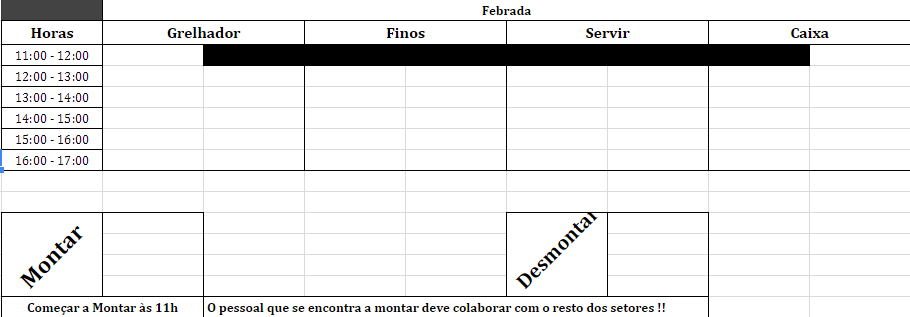
\includegraphics[width=0.88\textwidth]{imagens/escalas.png}
        \item Ligar a máquina de finos à corrente pelo menos um dia antes da febrada, para garantir que esta refresca.
        \item Pedir trocos ao Tesoureiro o quanto antes, para ter caixa inicial.
        \item Senhas e preçário: é essencial fazer senhas para cada evento específico, imprimi-las e cortá-las, bem como imprimir o preçário, que é discutido primeiro com o Tesoureiro. Não se esqueçam de rasgar e deitar as senhas ao lixo assim que as recebam durante a febrada para impedir as habituais borlas.
    \end{itemize}

    \item O dia da febrada
    \begin{itemize}
        \item Se forem seguidos todos os passos acima terão uma febrada de sucesso e neste dia só precisam de ir buscar as febras e o pão entretanto encomendados, montar a tenda e temperar as febras.
        \item Tempero das febras: juntem toda a carne num alguidar e deitem bastante massa de alho, pimentão doce, ervas de Provence, pimenta branca, sal e por fim, um fino. Usem luvas!
        \item É importante terem febras prontas antes da hora de afluência (meio-dia quando as mesmas são à hora de almoço), de modo a que não existam filas à hora de almoço e tudo flua super-rápido.
        \item No fim, deixem tudo limpo e arrumado e se ainda houver cerveja no barril, façam bar aberto a troco de um preço reduzido, as pessoas gostam e de outra maneira a cerveja iria para o lixo. O mesmo se aplica à carne e ao pão. Tentem sempre não desperdiçar.
        \item Caso sobre pão, contactem uma instituição de recolha de comida, que fará a recolha de imediato.
    \end{itemize}
\end{itemize}